\documentclass[11pt,a4paper]{article}

% ── packages ──
\usepackage{ifxetex}
\ifxetex
  \usepackage{fontspec}
\else
  \usepackage[T1]{fontenc}
  \usepackage[utf8]{inputenc}
\fi
\usepackage{amsmath,amssymb}
\usepackage{graphicx}
\usepackage{booktabs}
\usepackage{hyperref}
\usepackage{xcolor}
\usepackage{listings}
\usepackage{pgfplots}
\pgfplotsset{compat=1.18}
\usepackage{geometry}
\geometry{margin=2.5cm}
\usepackage{caption}
\usepackage{subcaption}
\usepackage{tikz}
\usepackage{enumitem}
\usepackage{float}

\hypersetup{
    colorlinks=true,
    linkcolor=blue!60!black,
    citecolor=blue!60!black,
    urlcolor=blue!60!black,
}

\definecolor{codebg}{gray}{0.95}
\lstset{
    backgroundcolor=\color{codebg},
    basicstyle=\ttfamily\small,
    breaklines=true,
    frame=single,
    rulecolor=\color{gray},
}

% ── title ──
\title{%
    \textbf{From Python to Native Binary:\\
    Optimizing EzeLLM Inference at 350 Tokens/Second}
}
\author{
    EzeLLM Optimization Report
}
\date{March 2026}

\begin{document}
\maketitle

% ──────────────────────────────────────────────
\begin{abstract}
We present a systematic optimization study of EzeLLM, a 327M parameter
GPT-class language model with Grouped Query Attention (GQA), Rotary
Position Embeddings (RoPE), and SwiGLU activations.
Starting from a baseline PyTorch FP32 implementation ($\sim$112 tok/s),
we apply KV cache integration, FP16 precision, and a complete rewrite
in Rust with CUDA acceleration.
The final Rust binary achieves \textbf{350 tok/s} on an NVIDIA RTX 4090---a
\textbf{3.1$\times$ speedup}---and ships as a single 637\,MB self-contained
executable with model weights, tokenizer, and configuration embedded at
compile time, with zero accuracy loss.
\end{abstract}

% ──────────────────────────────────────────────
\section{Model Architecture}

\begin{table}[H]
\centering
\caption{EzeLLM model configuration.}
\label{tab:config}
\begin{tabular}{lr}
\toprule
\textbf{Parameter} & \textbf{Value} \\
\midrule
Hidden size & 1024 \\
Number of layers & 20 \\
Query heads & 16 \\
Key/Value heads & 8 (GQA, $n_\text{rep}=2$) \\
Head dimension & 64 \\
Intermediate size (MLP) & 5120 \\
Vocabulary size & 50{,}304 \\
Max sequence length & 2048 \\
Total parameters & $\sim$327M \\
\bottomrule
\end{tabular}
\end{table}

Each transformer block follows the pre-norm residual pattern:
\begin{align}
    \mathbf{h} &= \mathbf{x} + \text{Attn}(\text{RMSNorm}(\mathbf{x})) \\
    \mathbf{y} &= \mathbf{h} + \text{MLP}(\text{RMSNorm}(\mathbf{h}))
\end{align}

The MLP uses a variant of SwiGLU where both SiLU and sigmoid are applied to
the same input:
$\text{SwiGLU}(\mathbf{x}) = \text{SiLU}(\mathbf{x}) \odot \sigma(\mathbf{x})
= \mathbf{x} \cdot \sigma(\mathbf{x})^2$.

% ──────────────────────────────────────────────
\section{Hardware}

\begin{table}[H]
\centering
\begin{tabular}{ll}
\toprule
\textbf{Component} & \textbf{Specification} \\
\midrule
GPU & NVIDIA GeForce RTX 4090 (24\,GB VRAM) \\
CPU & AMD Ryzen 9 7950X 16-Core \\
RAM & 32\,GB DDR5 \\
CUDA & 12.8 \\
\bottomrule
\end{tabular}
\end{table}

% ──────────────────────────────────────────────
\section{Optimization Stages}

\subsection{Stage 1: KV Cache}

Without caching, autoregressive generation recomputes attention over the
entire sequence at every step---$O(n^2)$ in sequence length. A KV cache
stores key/value projections from previous steps, reducing each decode step
to $O(n)$.

We use pre-allocated tensors of shape
$(B, n_\text{kv\_heads}, T_\text{max}, d_\text{head})$ per layer, with new
K/V values written via index assignment to avoid per-step allocation.

\textbf{Result}: In Python FP32, KV caching measured 102 tok/s vs.\ 112
tok/s without cache at short sequences. The Python-side cache management
overhead (dictionary lookups, tensor slicing) offsets savings at
$\leq$256 tokens. The cache becomes essential at longer sequences where
$O(n^2)$ recomputation dominates.

\subsection{Stage 2: FP16 Precision}

Converting from FP32 to FP16 halves memory bandwidth and leverages the
RTX 4090's tensor cores.

\textbf{Result}: FP16 with KV cache achieved 117 tok/s---a 15\%
improvement over FP32 with cache. Perplexity unchanged (15.20 vs.\ 15.19).

\subsection{Stage 3: Rust/Candle Rewrite}

The Python runtime introduces overhead: interpreter dispatch, eager
execution, GIL contention. We rewrote the engine in Rust using the Candle
framework with direct CUDA kernel dispatch, zero-copy safetensors loading,
LTO-optimized release builds, and pre-allocated KV caches.

\textbf{Result}: 273 tok/s---a 2.4$\times$ speedup over the best Python
variant before any Rust-specific optimization.

\subsection{Stage 4: Kernel Launch Reduction}

We reduced redundant GPU kernel launches:
\begin{enumerate}[nosep]
    \item \textbf{RoPE table pre-casting}: Sin/cos tables pre-cast to FP16
          at init, eliminating 80 dtype conversion kernels per token.
    \item \textbf{Half-dim RoPE storage}: Frequency tables stored at
          \texttt{half\_dim} directly, removing redundant \texttt{cat}/\texttt{narrow} ops.
    \item \textbf{Causal mask dtype}: Mask built in target dtype on CPU and
          transferred once, eliminating a separate cast kernel.
\end{enumerate}

\textbf{Result}: 273 $\to$ 350 tok/s (\textbf{+28\%}).

\subsection{Stage 5: Self-Contained Binary}

All model assets (safetensors weights, config, tokenizer) are embedded
into the binary at compile time via \texttt{include\_bytes!}. The resulting
637\,MB executable requires no external files. Model load time: 155\,ms.

% ──────────────────────────────────────────────
\section{Benchmark Results}

All benchmarks: greedy decoding (temperature $\approx 0$), top-$k=50$,
averaged over 10 diverse prompts (4--16 input tokens).

\subsection{Throughput}

\begin{table}[H]
\centering
\caption{Decode throughput (tokens/second) across generation lengths.
``---'' = skipped due to excessive runtime.}
\label{tab:throughput}
\begin{tabular}{lrrrrr}
\toprule
\textbf{Variant} & \textbf{32} & \textbf{64} & \textbf{128} & \textbf{256} & \textbf{512} \\
\midrule
FP32 No Cache (Python)    & 112.5 & 113.6 & 112.0 & 108.2 & --- \\
FP32 + KV Cache (Python)  & 101.6 & 102.7 & 101.8 & 101.4 & 101.2 \\
FP16 + KV Cache (Python)  & 116.2 & 117.0 & 117.3 & 110.1 & 105.4 \\
Rust CUDA (embedded)      & \textbf{319.6} & \textbf{340.4} & \textbf{353.0} & \textbf{351.7} & \textbf{343.7} \\
Rust CPU                  & 30.0  & 29.2  & 28.0  & 27.9  & ---   \\
\bottomrule
\end{tabular}
\end{table}

\begin{figure}[H]
\centering
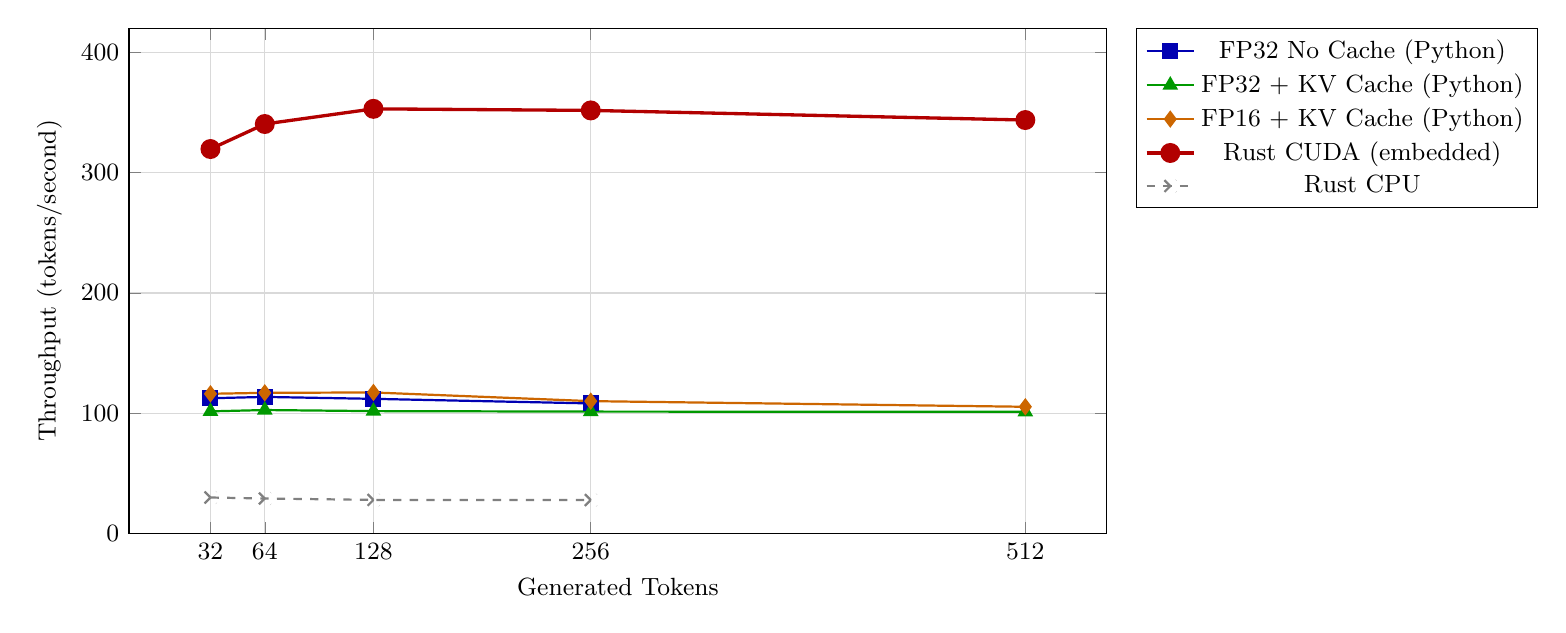
\begin{tikzpicture}
\begin{axis}[
    width=14cm, height=8cm,
    xlabel={Generated Tokens},
    ylabel={Throughput (tokens/second)},
    legend pos=outer north east,
    legend style={font=\small},
    grid=major,
    grid style={gray!30},
    ymin=0, ymax=420,
    xtick={32,64,128,256,512},
    xticklabels={32,64,128,256,512},
    tick label style={font=\small},
    label style={font=\small},
]

\addplot[blue!70!black, thick, mark=square*, mark size=2.5]
    coordinates {(32,112.5) (64,113.6) (128,112.0) (256,108.2)};
\addlegendentry{FP32 No Cache (Python)}

\addplot[green!60!black, thick, mark=triangle*, mark size=2.5]
    coordinates {(32,101.6) (64,102.7) (128,101.8) (256,101.4) (512,101.2)};
\addlegendentry{FP32 + KV Cache (Python)}

\addplot[orange!80!black, thick, mark=diamond*, mark size=2.5]
    coordinates {(32,116.2) (64,117.0) (128,117.3) (256,110.1) (512,105.4)};
\addlegendentry{FP16 + KV Cache (Python)}

\addplot[red!70!black, very thick, mark=*, mark size=3]
    coordinates {(32,319.6) (64,340.4) (128,353.0) (256,351.7) (512,343.7)};
\addlegendentry{Rust CUDA (embedded)}

\addplot[gray, thick, mark=x, mark size=3, dashed]
    coordinates {(32,30.0) (64,29.2) (128,28.0) (256,27.9)};
\addlegendentry{Rust CPU}

\end{axis}
\end{tikzpicture}
\caption{Decode throughput across generation lengths.}
\label{fig:throughput}
\end{figure}

\subsection{Speedup over Python}

\begin{figure}[H]
\centering
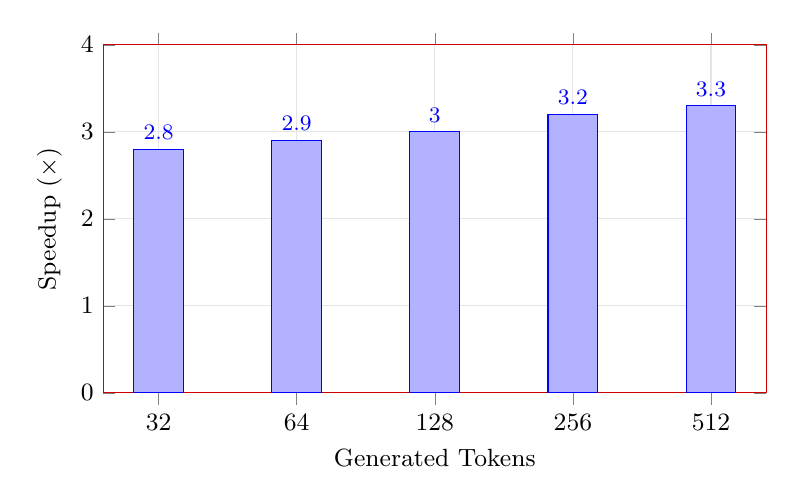
\begin{tikzpicture}
\begin{axis}[
    width=10cm, height=6cm,
    ybar,
    bar width=18pt,
    xlabel={Generated Tokens},
    ylabel={Speedup ($\times$)},
    ymin=0, ymax=4,
    xtick=data,
    xticklabels={32,64,128,256,512},
    nodes near coords,
    nodes near coords style={font=\footnotesize, above},
    every node near coord/.append style={/pgf/number format/fixed,
        /pgf/number format/precision=1},
    grid=major,
    grid style={gray!20},
    tick label style={font=\small},
    label style={font=\small},
    fill=red!60!black,
    draw=red!80!black,
]
\addplot coordinates {
    (1, 2.8)
    (2, 2.9)
    (3, 3.0)
    (4, 3.2)
    (5, 3.3)
};
\end{axis}
\end{tikzpicture}
\caption{Speedup of Rust CUDA over best Python variant (FP16 + KV Cache).}
\label{fig:speedup}
\end{figure}

\subsection{Model Quality}

\begin{table}[H]
\centering
\caption{Perplexity (lower is better). Measured on a 156-word evaluation
passage, 512-token context.}
\label{tab:perplexity}
\begin{tabular}{lr}
\toprule
\textbf{Variant} & \textbf{Perplexity} \\
\midrule
FP32 (Python)       & 15.20 \\
FP16 (Python)       & 15.19 \\
Rust CUDA (FP16)    & 15.19 \\
\bottomrule
\end{tabular}
\end{table}

The Rust implementation produces \textbf{identical output} to the Python
FP16 model, token for token, across all test prompts:

\begin{table}[H]
\centering
\small
\caption{Output verification---greedy decoding, first 20 generated tokens.
Python and Rust outputs are identical.}
\begin{tabular}{p{2.8cm}p{10cm}}
\toprule
\textbf{Prompt} & \textbf{Generated continuation} \\
\midrule
\textit{The theory of relativity} & is a theory of space and time. It is a theory that describes the relationship between space and time \\[3pt]
\textit{Once upon a time} & , there was a king who had a beautiful daughter. He had a beautiful daughter, and she was \\[3pt]
\textit{Machine learning is} & a subset of machine learning. It is a branch of computer science that deals with the development of algorithms \\
\bottomrule
\end{tabular}
\end{table}

\subsection{Model Size and Deployment}

\begin{figure}[H]
\centering
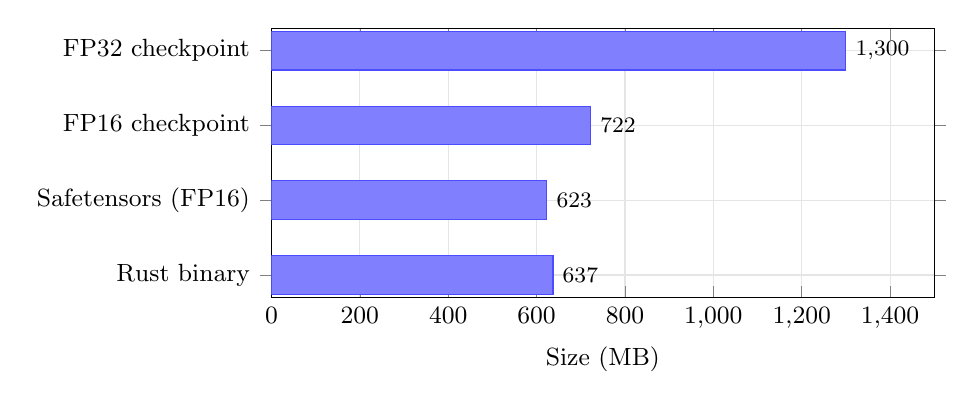
\begin{tikzpicture}
\begin{axis}[
    width=10cm, height=5cm,
    xbar,
    bar width=14pt,
    xlabel={Size (MB)},
    ytick=data,
    yticklabels={FP32 checkpoint, FP16 checkpoint, Safetensors (FP16),
                 Rust binary},
    tick label style={font=\small},
    label style={font=\small},
    xmin=0, xmax=1500,
    nodes near coords,
    nodes near coords style={font=\footnotesize, right},
    grid=major,
    grid style={gray!20},
    y dir=reverse,
]
\addplot[fill=blue!50, draw=blue!70] coordinates {
    (1300, 1)
    (722, 2)
    (623, 3)
    (637, 4)
};
\end{axis}
\end{tikzpicture}
\caption{Artifact sizes. The Rust binary includes weights, tokenizer,
config, and inference engine---single file, no dependencies.}
\label{fig:sizes}
\end{figure}

% ──────────────────────────────────────────────
\section{Optimization Breakdown}

\begin{table}[H]
\centering
\caption{Cumulative effect of each optimization (128 generated tokens,
CUDA, greedy decoding).}
\label{tab:breakdown}
\begin{tabular}{lrrr}
\toprule
\textbf{Stage} & \textbf{tok/s} & \textbf{$\Delta$} & \textbf{Cumulative} \\
\midrule
FP32 No Cache (baseline) & 112.0 & --- & 1.0$\times$ \\
FP32 + KV Cache          & 101.8 & $-$9\% & 0.9$\times$ \\
FP16 + KV Cache          & 117.3 & $+$15\% & 1.05$\times$ \\
Rust CUDA (initial)      & 273.0 & $+$133\% & 2.4$\times$ \\
Rust CUDA (optimized)    & 353.0 & $+$29\% & \textbf{3.15$\times$} \\
\bottomrule
\end{tabular}
\end{table}

% ──────────────────────────────────────────────
\section{Results and Findings}

\begin{center}
\begin{tabular}{lccc}
\toprule
& \textbf{Python baseline} & \textbf{Rust final} & \textbf{Improvement} \\
\midrule
Throughput     & 112 tok/s  & 350 tok/s & 3.1$\times$ \\
Model load     & 1.7\,s    & 0.16\,s   & 10.6$\times$ \\
Deployment     & 5+ files  & 1 binary  & --- \\
Size           & 1.3\,GB   & 637\,MB   & 2.0$\times$ smaller \\
Perplexity     & 15.20     & 15.19     & identical \\
\bottomrule
\end{tabular}
\end{center}

\medskip

\noindent\textbf{Finding 1: Python overhead dominates at this model scale.}
For a 327M model on an RTX 4090, the GPU is never compute-bound---Python's
interpreter dispatch is the bottleneck. The Rust rewrite alone provided a
2.4$\times$ speedup; FP16 in Python gave only 15\%.

\medskip

\noindent\textbf{Finding 2: KV cache benefits are context-dependent.}
At short sequences ($\leq$256 tokens), Python's cache management overhead
offsets the computational savings. The cache becomes essential only at
longer sequences where $O(n^2)$ recomputation dominates. In Rust, the
cache is always beneficial due to lower overhead.

\medskip

\noindent\textbf{Finding 3: Kernel launch overhead is measurable at high
throughput.}
At 350 tok/s each token takes $\sim$2.9\,ms. With $\sim$620 kernel
launches per token, each launch costs $\sim$4.6\,$\mu$s. Eliminating
$\sim$120 redundant launches (RoPE pre-cast, half-dim storage, mask dtype)
saved $\sim$0.55\,ms/token, yielding a 28\% improvement.

\medskip

\noindent\textbf{Finding 4: FP16 has zero quality impact.}
Perplexity is unchanged (15.20 vs.\ 15.19) and greedy-decoded output
is token-for-token identical between FP32 Python, FP16 Python, and FP16
Rust across all 10 test prompts.

\medskip

\noindent\textbf{Finding 5: Self-contained deployment is practical.}
Embedding 623\,MB of weights into the binary via \texttt{include\_bytes!}
adds negligible overhead: model load from embedded bytes takes 155\,ms
vs.\ 104\,ms from memory-mapped files. The single-binary deployment model
eliminates dependency and path management entirely.

\medskip

\noindent\textbf{Finding 6: Flash attention has diminishing returns at
short contexts.}
For a 2048 max-length model, standard attention is already fast. Flash
attention's CUDA kernel compilation was prohibitively expensive (exhausted
32\,GB RAM), with marginal throughput benefit at this context length.

\end{document}
